\chapter{Multiscale turbulence measurements}
\label{ch:TurbulenceMeasurements}
Development of a first-principles understanding
of turbulent transport in a tokamak
requires multi-tiered validation\ldots
comparing not just heat fluxes, but
also turbulent spectra etc.
\diiid's extensive suite of fluctuation diagnostics
provides an ideal setting to validate
predicted changes~\cite{howard_pp16}
to turbulent spectra when altering relative drive
between electron-scale and ion-scale turbulence.


\section{Overview of multiscale gyrokinetic predictions}


\section{Experimental conditions}
The experiment was run in the ITER-similar shape,
with aspect ratio, elongation, and triangularity
all closely matched to those of the ITER-baseline scenario
\cite[Sec.~13.5 \& 13.6]{wesson}.
The on-axis toroidal field $B_T = \SI{1.7}{\tesla}$ and
plasma current $I_p = \SI{1.3}{\mega\ampere}$
produced $q_{95} = 3.15$,
where $q_{95}$ is the average value
of the safety factor $q$~\cite[Sec.~3.4]{wesson}
over the surface that encloses $95\%$
of the poloidal flux within the last-closed flux surface.
The neutral beams~\cite[Sec.~5.3-5.5]{wesson}
were operated with feedback to maintain
$\beta_N = 1.9$, where
$\beta_N$ is the normalized plasma pressure~\cite[Sec.~6.18]{wesson}.
In order to suppress core MHD,
an average neutral-beam torque of $\sim \SI{1.5}{\newton \meter}$
was injected into the plasma;
note that this is $\sim 4\times$ larger than
the projected ITER-equivalent torque~\cite{garofalo_nf11}.
In order to alter the local electron-scale and ion-scale drives,
the electron cyclotron resonance heating (ECH)~\cite[Sec.~5.10]{wesson}
location was scanned between $\rho = 0.5$ and $\rho = 0.8$,
where $\rho$ is the square root of the normalized toroidal flux
(which scales as $r / a$, with
$r$ being the minor-radial coordinate and
$a$ being the minor radius of the plasma).
Intra-shot scans of the ECH location
were plagued with core MHD, so
only shot-to-shot, MHD-free scans of the ECH location
are considered here.
The line-averaged density was
$\bar{n}_e = \SI{5.2e19}{\per\meter\cubed}$.
Impurities are removed from the plasma
by both large and small edge localized modes (ELMs)~\cite[Sec.~7.17]{wesson}.
The time histories of several actuators and plasma parameters
are shown in Figure~\ref{fig:TurbulenceMeasurements:traces}.
Note that multiscale gyrokinetic simulations
of this experiment's reference discharge,
\diiid\space shot $153523$ with ECH at $\rho = 0.5$,
indicate that the turbulent transport
is intrinsically multiscale in nature~\cite{holland_nf17}.

\begin{figure}
  \centering
  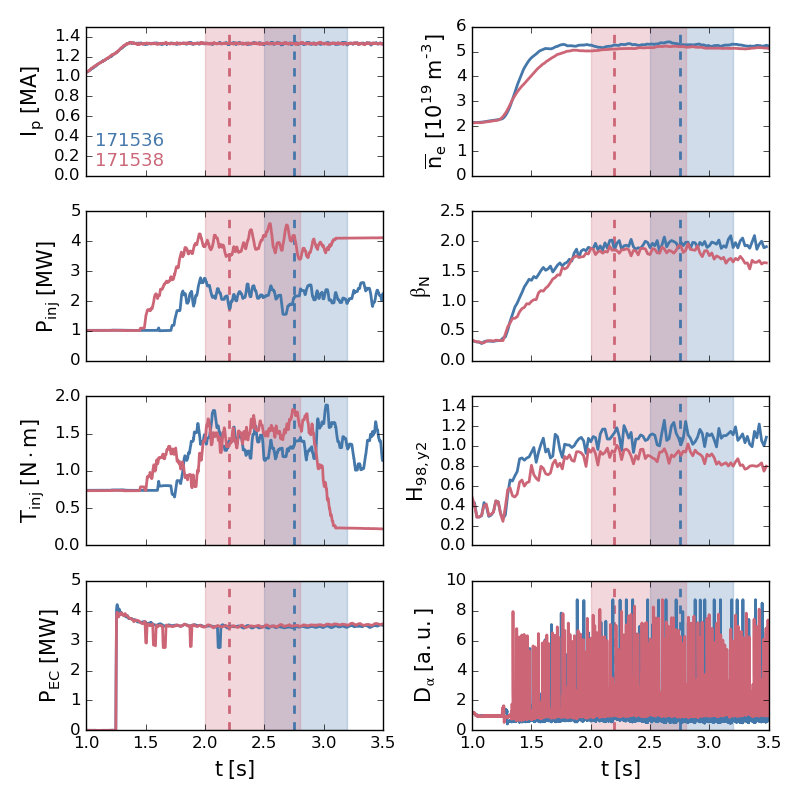
\includegraphics[width = \textwidth]{%
    Chapters/TurbulenceMeasurements/figs/traces.png}
  \caption[Time histories of various actuators \& plasma parameters]{%
    Time histories of various actuators and plasma parameters:
    (a) plasma current $I_p$,
    (b) neutral beam injected (NBI) power $P_{\text{inj}}$,
    (c) NBI torque $T_{\text{inj}}$,
    (d) electron cyclotron resonance heating (ECH) power $P_{\text{ECH}}$,
    (e) line-averaged density $\bar{n}_e$,
    (f) normalized plasma pressure $\beta_N$,
    (g) confinement quality $H_{98,\text{y}2}$, and
    (h) divertor $D_{\alpha}$ light, indicating
    the presence of large and small edge localized modes (ELMs).
    The ECH heating location was
    at $\rho = 0.5$ in $171536$ and
    at $\rho = 0.8$ in $171538$.
  }
\label{fig:TurbulenceMeasurements:traces}
\end{figure}

Equilibrium profiles
\begin{itemize}
  \item averaging over \textcolor{red}{XXX ms}
  \item What types of fits? (splines, RBF, etc.)
  \item Electron-density profiles -- Thomson w/ CO$_2$ normalization?
    Reflectometer?
  \item Electron-temperature profiles -- Thomson \& ECE (or ECE cutoff?)
  \item Ion-temperature profiles -- \textcolor{red}{???}
  \item CER provides C$^{6+}$ density, temperature, and rotation
  \item $E_r$ computed using force balance for
    C$^{6+}$ pressure and toroidal rotation.
    \textcolor{red}{poloidal rotation neglected?}
  \item \textcolor{red}{MSE-constrained EFIT? Kinetic?}
  \item \textcolor{red}{How are ELMs handled?}
  \item Uncertainties
  \item Clear change in turbulent drives with ECH location
  \item The profiles are shown in
    Figure~\ref{fig:TurbulenceMeasurements:profiles}.
\end{itemize}

\begin{figure}
  \centering
  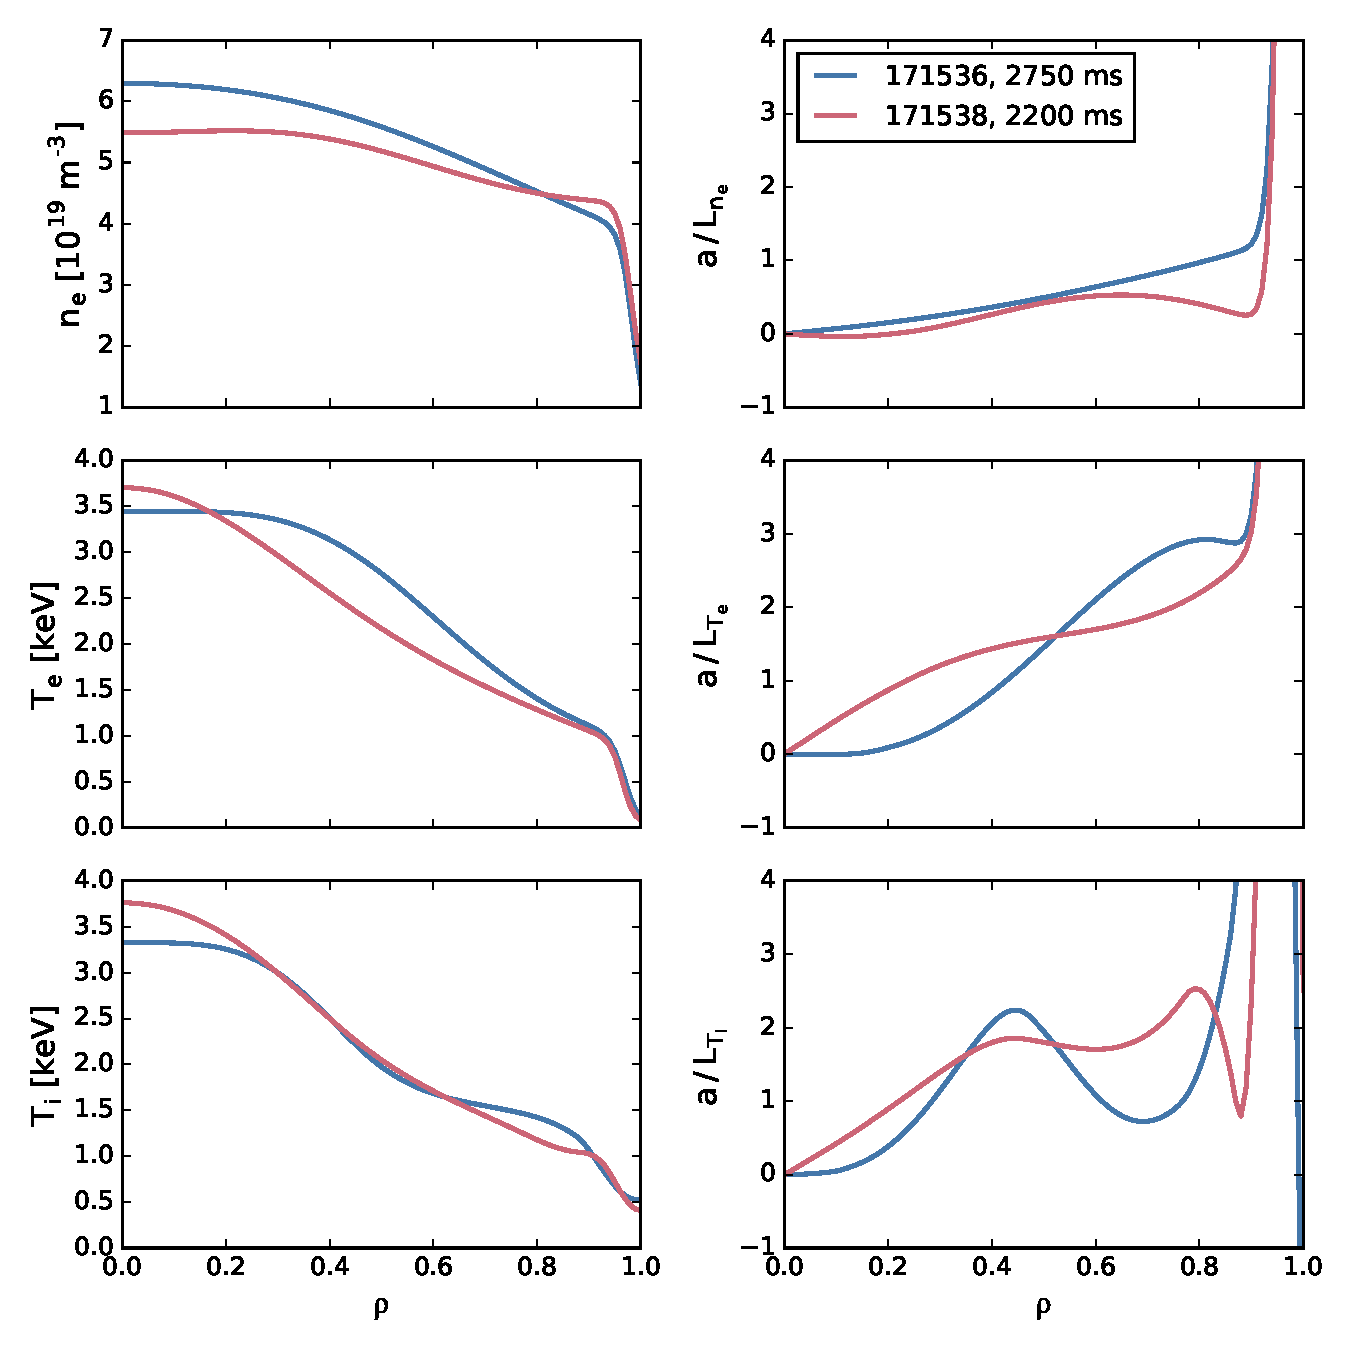
\includegraphics[width = \textwidth]{%
    Chapters/TurbulenceMeasurements/figs/profiles.pdf}
  \caption[Equilibrium profiles, inverse scale lengths, \& $\ExB$ shearing rate]{%
    Profiles, inverse scale lengths, and $\ExB$ shearing rate:
    (a) electron density $n_e$,
    (b) electron temperature $T_e$,
    (c) deuterium temperature $T_i$,
    (d) radial electric field $E_r$ along the outboard midplane,
    (e) normalized inverse $n_e$ scale length $a / L_{n_e}$,
    (f) normalized inverse $T_e$ scale length $a / L_{T_e}$,
    (g) normalized inverse $T_i$ scale length $a / L_{T_i}$,
    (h) $\ExB$ shearing rate $\gamma_E$.
    The ECH heating location was
    at $\rho = 0.5$ in $171536$ and
    at $\rho = 0.8$ in $171538$.
  }
\label{fig:TurbulenceMeasurements:profiles}
\end{figure}


\section{Combined PCI-interferometer measurements}
\label{sec:TurbulenceMeasurements:Measurements}


\subsection{ELM filtering}
\label{sec:TurbulenceMeasurements:ELM_filtering}
Edge localized modes (ELMs) expel impurities from the plasma but
will also present severe challenges to plasma-facing components
in future reactors~\cite[Sec.~7.17]{wesson}.
Because of their virulence and their bursty nature,
ELMs produce strong spiking in the interferometer and PCI measurements,
whitening the measured spectra
[Sec.~10.3.2.3]\cite{bendat_and_piersol}.
Additionally, the temperature and density profiles relax during an ELM,
altering the turbulent drives in the plasma edge.
In order to accurately estimate
the spectrum of the background turbulence, then,
the ELM contributions to the interferometer and PCI measurements
must be removed.

\begin{figure}
  \centering
  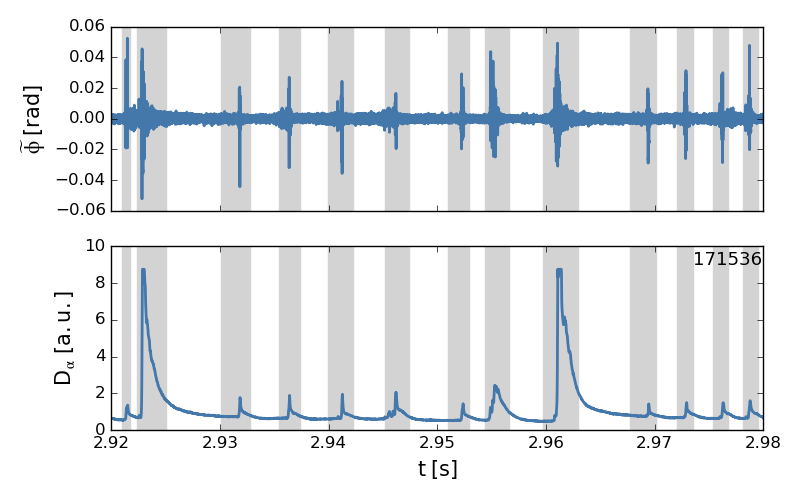
\includegraphics[width = \textwidth]{%
    Chapters/TurbulenceMeasurements/figs/ELM_filtering_example.png}
  \caption[ELM filtering]{%
    Edge localized modes (ELMs) must be removed
    from the PCI and interferometer measurements
    prior to spectral analysis of the background turbulence.
    (Upper panel): The interferometer-measured
    fluctuating phase $\tilde{\phi}$,
    with large, ELM-induced spiking.
    (Lower panel): Divertor $D_{\alpha}$ emission,
    indicating the presence of large Type I ELMs
    as well as smaller ELMs.
    Windows \emph{excluded} from spectral analysis are shown in gray.
    The \diiid\space shot number is shown in the upper right
    of the lower panel.
  }
\label{fig:TurbulenceMeasurements:ELM_filtering_example}
\end{figure}

In this work, ELMs are simply and automatically detected
using measurements from the interferometer.
After the high-pass filtering described in
Section~\ref{sec:Implementation:DataPreparation:high_pass_filtering},
the interferometer-measured fluctuating phase $\tilde{\phi}$
is a zero-mean, random process,
as shown in the upper panel of
Figure~\ref{fig:TurbulenceMeasurements:ELM_filtering_example}.
Large, intermittent spikes pepper $\tilde{\phi}(t)$ during ELMy H-mode, and
the lower panel of
Figure~\ref{fig:TurbulenceMeasurements:ELM_filtering_example}
indicates that these spikes are well correlated
with ELM-induced $D_{\alpha}$ emission in the divertor.
While the $D_{\alpha}$ emission following large Type I ELMs
exhibits a relatively slow decay,
the interferometer-measured $\tilde{\phi}$
returns to stationarity much more rapidly.
Thus, it is desirable to identify
stationary inter-ELM windows
from the interferometer measurements
rather than the $D_{\alpha}$ emission.
Points in the interferometer-measured $\tilde{\phi}$
exceeding $3 \times$ the RMS value
are identified as ELMs, and
successive ELMs are required to be separated
by at least a $\SI{0.5}{\milli\second}$ ``debouncing time''
(spikes separated by less than the debouncing time
are classified as belonging to the same ELM).
Subsequent spectral analysis is then performed
using only the $20\%$ -- $80\%$ inter-ELM windows
of the interferometer and PCI measurements.
Figure~\ref{fig:TurbulenceMeasurements:ELM_filtering_example}
shows the windows \emph{excluded} from spectral analysis in gray.


\subsection{Frequency spectra}
\label{sec:TurbulenceMeasurements:Sf}
\begin{figure}
  \centering
  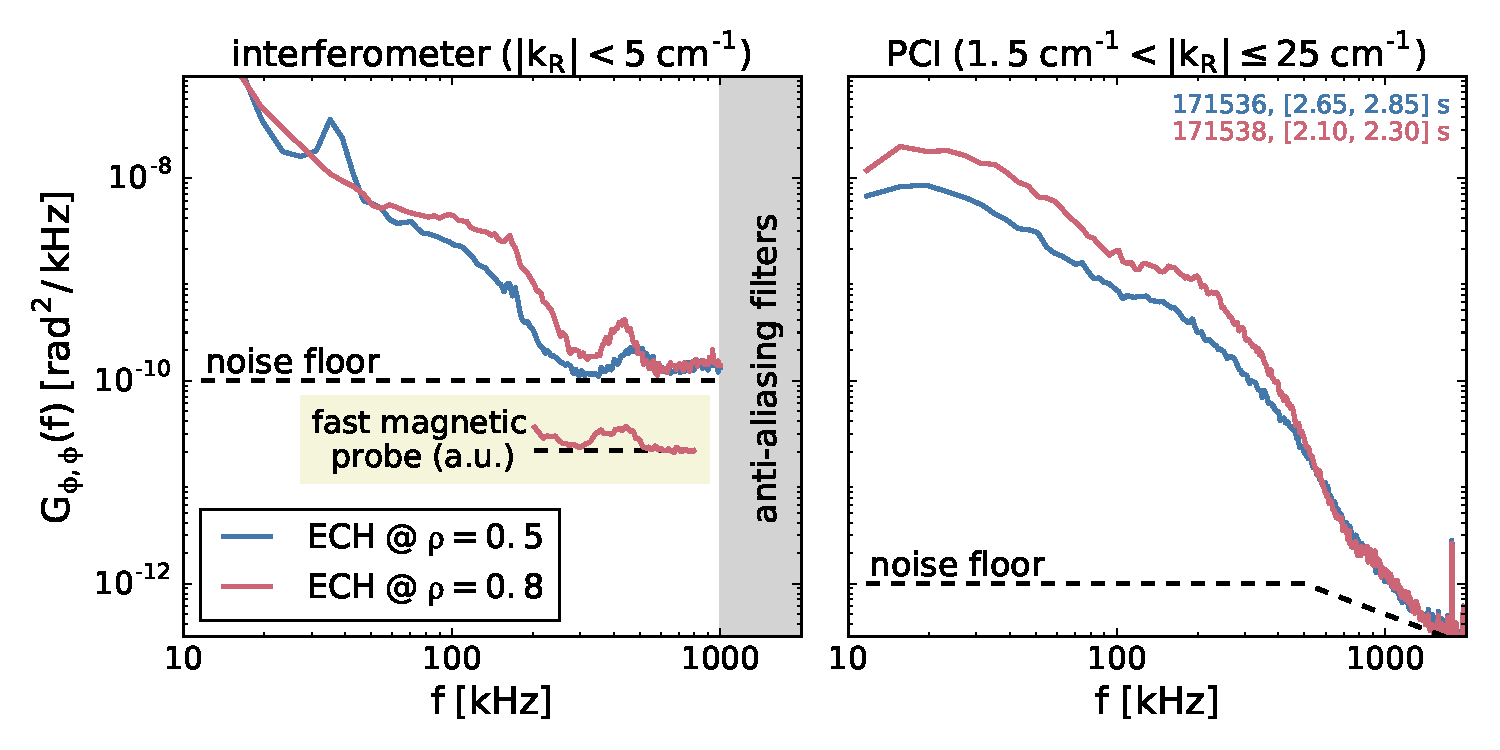
\includegraphics[width = \textwidth]{%
    Chapters/TurbulenceMeasurements/figs/Sf_interferometer_pci.pdf}
  \caption[Interferometer \& PCI frequency spectra]{%
    Interferometer and PCI frequency spectra.
  }
\label{fig:TurbulenceMeasurements:Sf_interferometer_pci}
\end{figure}
\begin{itemize}
  \item Coherence
  \item Collisionality
\end{itemize}


\subsection{Frequency-wavenumber spectra}
\label{sec:TurbulenceMeasurements:Skf}

\begin{figure}
  \centering
  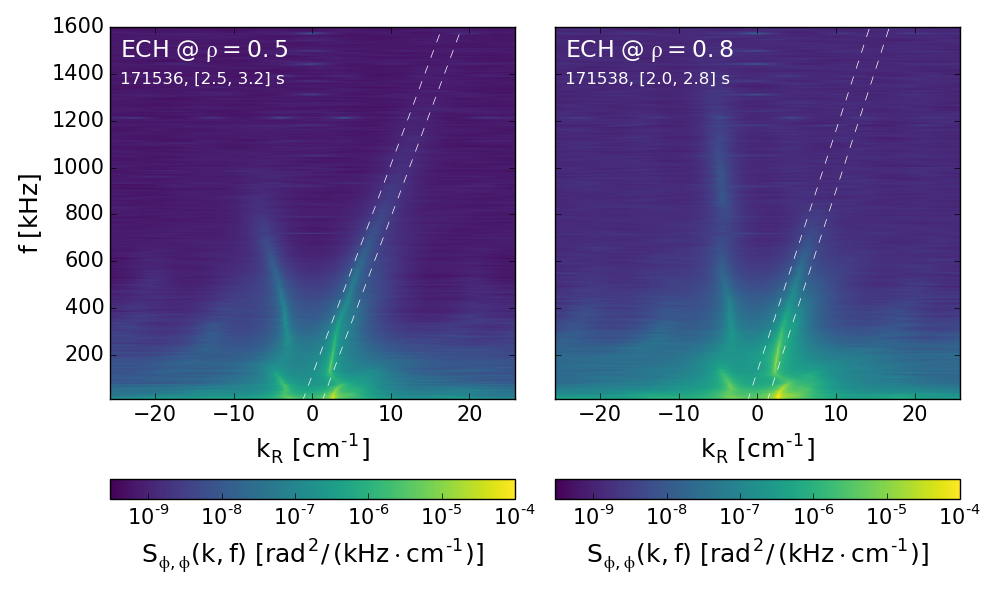
\includegraphics[width = \textwidth]{%
    Chapters/TurbulenceMeasurements/figs/Skf_pci.png}
  \caption[PCI frequency-wavenumber spectra]{%
    PCI frequency-wavenumber spectra. $p = 6$.
  }
\label{fig:TurbulenceMeasurements:Skf_pci}
\end{figure}


\subsection{Wavenumber spectra}
\label{sec:TurbulenceMeasurements:Sk}
\begin{figure}
  \centering
  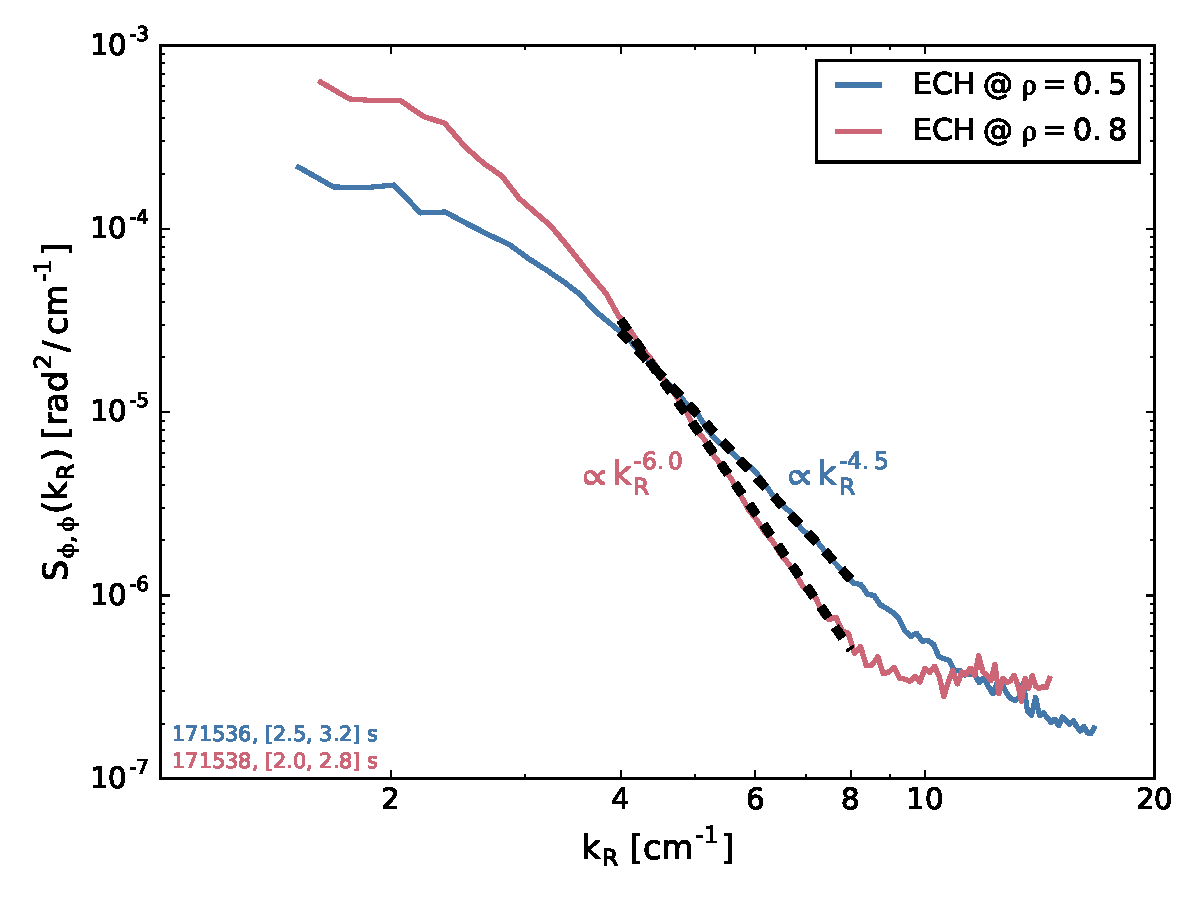
\includegraphics[width = 0.9 \textwidth]{%
    Chapters/TurbulenceMeasurements/figs/Sk_power_law.pdf}
  \caption[PCI-measured power law]{%
    PCI-measured power law from branches annotated in
    Figure~\ref{fig:TurbulenceMeasurements:Skf_pci}.
  }
\label{fig:TurbulenceMeasurements:Sk_power_law}
\end{figure}


\subsection{Doppler-shift localization of high-$k$ turbulence}
As a line-integrated measurement,
PCI is sensitive to fluctuations with wavevectors $\vect{k}$
that are perpendicular to the beam path
(i.e.\ $\vect{k} \perp \zhat$
for the vertical beam path of \diiid's PCI).
Further, fluctuations are strongly field-aligned
such that they are approximately perpendicular
to the local magnetic field;
assuming the fluctuations are electrostatic,
the local magnetic field is well-represented
by the equilibrium field $\Beq$ such that
$\vect{k} \perp \Beq$.
Thus, the wavevector satisfies
\begin{equation}
  \vect{k}
  \propto
  \zhat \cross \beq,
  \label{eq:TurbulenceMeasurements:kpropto}
\end{equation}
where $\beq = \Beq / |\Beq|$ is the unit vector
in the direction of the local equilibrium magnetic field.
Thus, the PCI-measured fluctuations have wavevectors
\begin{equation}
  \vect{k}
  =
  (\vect{k} \cdot \khat) \khat,
\end{equation}
where
\begin{equation}
  \khat
  =
  \frac{\zhat \cross \beq}{|\zhat \cross \beq|}
  \label{eq:TurbulenceMeasurements:khat}.
\end{equation}
For a tokamak with a dominant toroidal magnetic field,
$\beq \sim \zetahat$ and
$|\zhat \cross \beq| \sim 1$ such that
(\ref{eq:TurbulenceMeasurements:khat}) is never singular.
Noting the $(R, z, \zeta)$ and $(\rho, \theta, \zeta)$
coordinate systems defined in
Fig.~\ref{fig:TurbulenceMeasurements:coordinate_geometry} and
explicitly writing the equilibrium magnetic field
as the sum of its toroidal and poloidal components
$\Beq = B_{\zeta} \zetahat + B_{\theta} \thetahat$,
the unit vector (\ref{eq:TurbulenceMeasurements:khat})
can be explicitly written as
\begin{equation}
  \khat
  =
  \frac{%
    B_{\zeta} \Rhat + (B_{\theta} \sin\theta) \zetahat}{%
    {\left[ B_{\zeta}^2 + {(B_{\theta} \sin\theta)}^2 \right]}^{1/2}}.
  \label{eq:TurbulenceMeasurements:khat_explicit}
\end{equation}
Because $|B_{\theta}| \ll |B_{\zeta}|$,
the wavevectors are predominantly in the major-radial direction,
i.e.\ $\khat \sim \Rhat$.

\begin{figure}
  \centering
  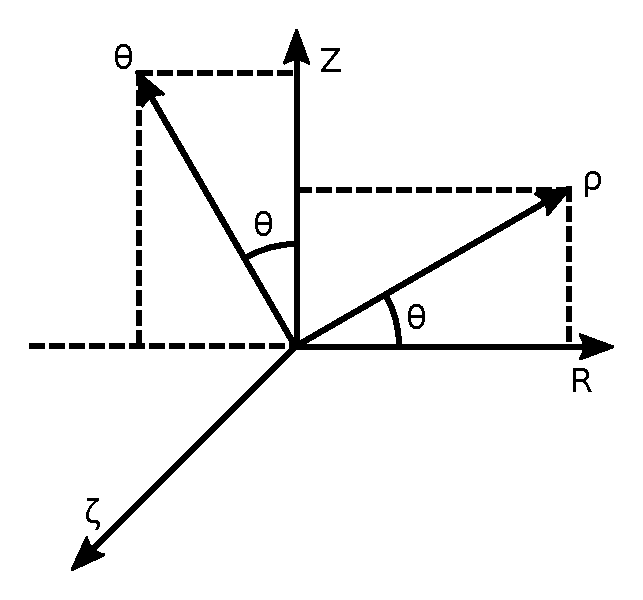
\includegraphics[width = 0.5 \textwidth]{%
    Chapters/TurbulenceMeasurements/figs/coordinate_geometry.pdf}
  \caption[Measurement coordinate system]{%
    Measurement coordinate system.
    Here, $R$ is the major-radial direction,
    $z$ is the lab-frame vertical direction,
    $\zeta$ is the toroidal angle,
    $\theta$ is the poloidal angle, and
    $\rho$ is a flux-surface label
    corresponding to the square root
    of the normalized toroidal magnetic-field flux.
  }
\label{fig:TurbulenceMeasurements:coordinate_geometry}
\end{figure}

Now, assuming that $\ExB$ advection
is the predominant contribution
to the PCI-measured phase velocity,
the line-integrated PCI measurements can be moderately localized.
To see this, note that the PCI measurements are Doppler shifted by
$\Delta \omega = \vect{k} \cdot \vect{v}$,
where $\vect{v}$ is the lab-frame velocity of the plasma.
Because $\vect{k} \perp \Beq$ by
(\ref{eq:TurbulenceMeasurements:kpropto}),
$\vect{k} \cdot \vect{v} = \vect{k} \cdot \vperp$, where
$\vperp$ is the velocity
perpendicular to the equilibrium magnetic field.
Defining the plasma frame via the ideal-MHD relation
$\vect{E} + \vperp \cross \Beq = 0$,
the perpendicular velocity is simply the $\ExB$ velocity
i.e.\ $\vperp = \vExB$.
Now, the electrostatic potential $\varphi = \varphi(\rho)$
is a flux function such that
the corresponding electric field is
$\vect{E} = -\nabla \varphi = E_r(\rho, \theta) \rhohat$.
The resulting $\ExB$ velocity is
\begin{align}
  \vExB
  =
  \frac{\vect{E} \times \Beq}{B_0^2}
  % \notag \\
  =
  \frac{E_r(\rho, \theta)}{B_0^2}
  \left(%
    B_{\theta} \zetahat
    -
    B_{\zeta} \thetahat
  \right)
  \label{eq:TurbulenceMeasurements:vExB}
\end{align}
such that the Doppler shift
$\Delta \omega = \vect{k} \cdot \vExB$ becomes
\begin{equation}
  \Delta \omega
  =
  \frac{%
    (\vect{k} \cdot \khat) E_r(\rho, \theta) \sin\theta}{%
    {\left[ B_{\zeta}^2 + {(B_{\theta} \sin\theta)}^2 \right]}^{1/2}}.
  \label{eq:TurbulenceMeasurements:Doppler_shift_from_ExB}
\end{equation}
Thus, the plasma's $\ExB$ rotation
results in a PCI-measured phase velocity
\begin{align}
  \vpciE
  =
  \frac{\Delta \omega}{k}
  =
  \frac{%
    \sgn(\vect{k} \cdot \khat) E_r(\rho, \theta) \sin\theta}{%
    {\left[ B_{\zeta}^2 + {(B_{\theta} \sin\theta)}^2 \right]}^{1/2}},
  \label{eq:TurbulenceMeasurements:PCI_phase_velocity_from_ExB}
\end{align}
where the sign function $\sgn(x)$
returns the sign of argument $x$.
Here, the plasma-frame phase velocity $v_{\text{ph}}$
of the fluctuations have been neglected,
which is valid when $|v_{\text{ph}}| \ll |\vpciE|$.
Further, note that the polarity of $\sin\theta$
switches at the plasma midplane (where $\theta = 0$) such that
(\ref{eq:TurbulenceMeasurements:PCI_phase_velocity_from_ExB})
switches signs when passing from above the plasma midplane
to below the plasma midplane.
Figure~\ref{fig:TurbulenceMeasurements:doppler_shift}
compares $\vpciE$ from
(\ref{eq:TurbulenceMeasurements:PCI_phase_velocity_from_ExB})
to the measured phase velocity $\vpcimeas$
of the high-$k$ turbulence observed in the left panel of
Figure~\ref{fig:TurbulenceMeasurements:Skf_pci}.

\begin{figure}
  \centering
  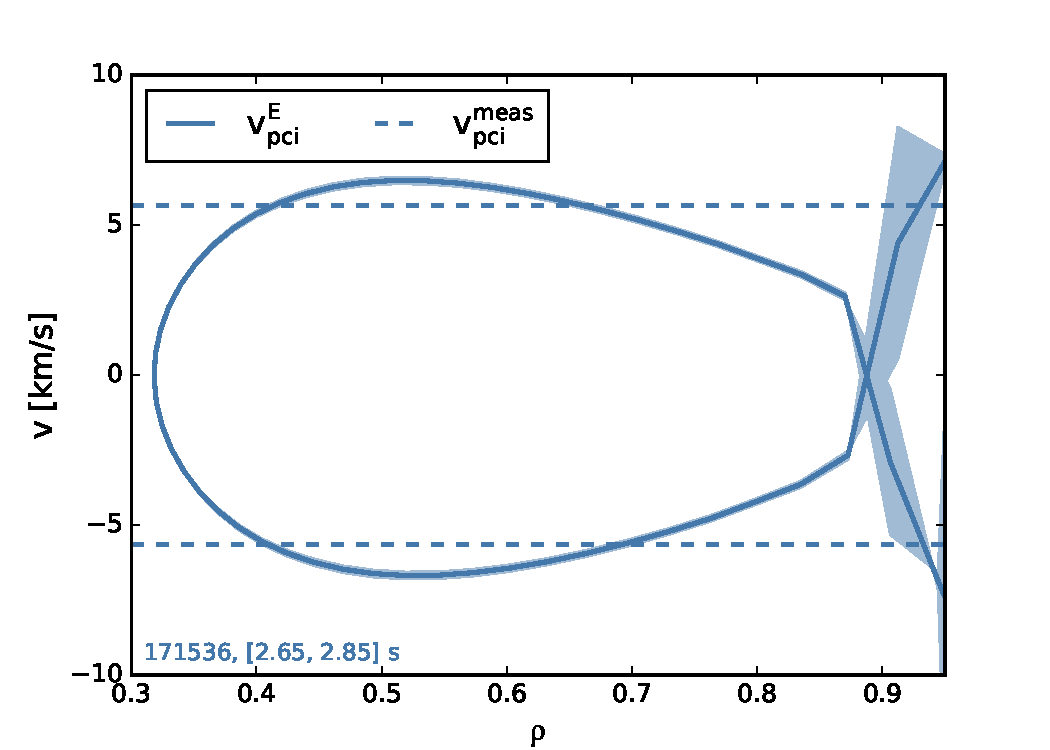
\includegraphics[width = 0.9 \textwidth]{%
    Chapters/TurbulenceMeasurements/figs/doppler_shift.pdf}
  \caption[Doppler-shift localization of high-$k$ turbulence]{%
    A comparison of the $\ExB$-induced phase velocity $\vpciE$ from
    (\ref{eq:TurbulenceMeasurements:PCI_phase_velocity_from_ExB})
    to the measured phase velocity $\vpcimeas$
    of the high-$k$ turbulence observed in the left panel
    of Figure~\ref{fig:TurbulenceMeasurements:Skf_pci}.
    The near degeneracy of $\vpciE$ with $\rho$
    corresponds to propagation above and below the plasma midplane.
    As the spatially filtering ``mask''~\cite{dorris_phd, dorris_rsi09}
    was not used in this experiment,
    it is not possible to determine whether
    $\vpcimeas$ corresponds to propagation above or below the midplane, so
    both $\vpcimeas$ and $-\vpcimeas$ are plotted.
  }
\label{fig:TurbulenceMeasurements:doppler_shift}
\end{figure}

As a brief aside, it should be emphasized
that the radial electric field $E_r$
in (\ref{eq:TurbulenceMeasurements:PCI_phase_velocity_from_ExB})
is \emph{not} a flux function.
To see this, recall that
the corresponding electrostatic potential
\emph{is} a flux function,
i.e.\ $\varphi = \varphi(\rho) = \varphi(\psi)$,
where $\psi$ is the flux-surface label
corresponding to the poloidal magnetic-field flux per radian.
Now,
\begin{align}
  E_r(\rho, \theta)
  &=
  -\left( \frac{\partial\varphi}{\partial r} \right)
  \notag \\
  &=
  -\left( \frac{d\varphi}{d\psi} \right)
  \left( \frac{\partial\psi}{\partial r} \right)
  \notag \\
  &=
  -\left( \frac{d\varphi}{d\psi} \right)
  \left( R B_{\theta} \right),
\end{align}
where the last line follows from the definition
of $\psi$ as the poloidal magnetic-field flux per radian.
The derivative $d\varphi / d\psi$
is a flux function because $\varphi$ is a flux function, and
this implies that $E_r / (R B_{\theta})$ is also a flux function.
Thus, the radial electric field at any point
within the last closed flux surface can be computed
from the radial electric field
along the outboard midplane (where $\theta = 0$) as follows
\begin{equation}
  \left.
  \frac{E_r}{R B_{\theta}}
  \right|_{\rho, \theta}
  =
  \left.
  \frac{E_r}{R B_{\theta}}
  \right|_{\rho, \theta = 0}.
  \label{eq:TurbulenceMeasurements:radial_electric_field}
\end{equation}


\section{TGLF modeling}
\begin{figure}[h!]
  \centering
  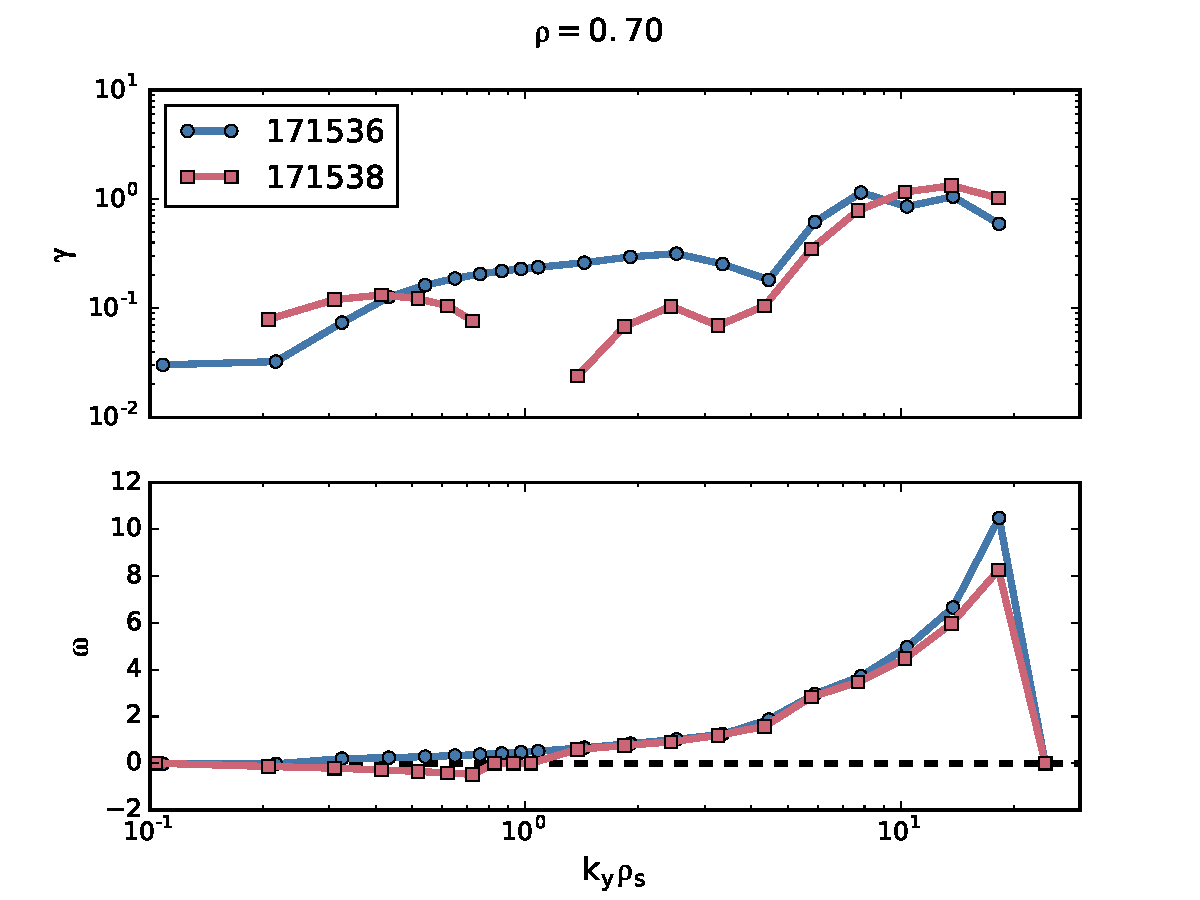
\includegraphics[width = \textwidth]{%
    Chapters/TurbulenceMeasurements/figs/linear_stability.pdf}
  \caption[Growth rates \& frequencies at $\rho=0.7$]{%
    Growth rates \& frequencies at $\rho=0.7$
    (i.e.\ we're slicing
    Figure~\ref{fig:TurbulenceMeasurements:TGLF_171536_vs_171538}
    at $\rho = 0.7$ for the most unstable mode, mode $1$).
    Note that only $171536$ uses SAT\_RULE $= 1$,
    which is calibrated against multiscale GYRO results;
    $171538$ uses SAT\_RULE $= 0$.
    Thus, it is difficult to draw conclusions\ldots
  }
\label{fig:TurbulenceMeasurements:linear_stability}
\end{figure}

\begin{figure}[h!]
  \centering
  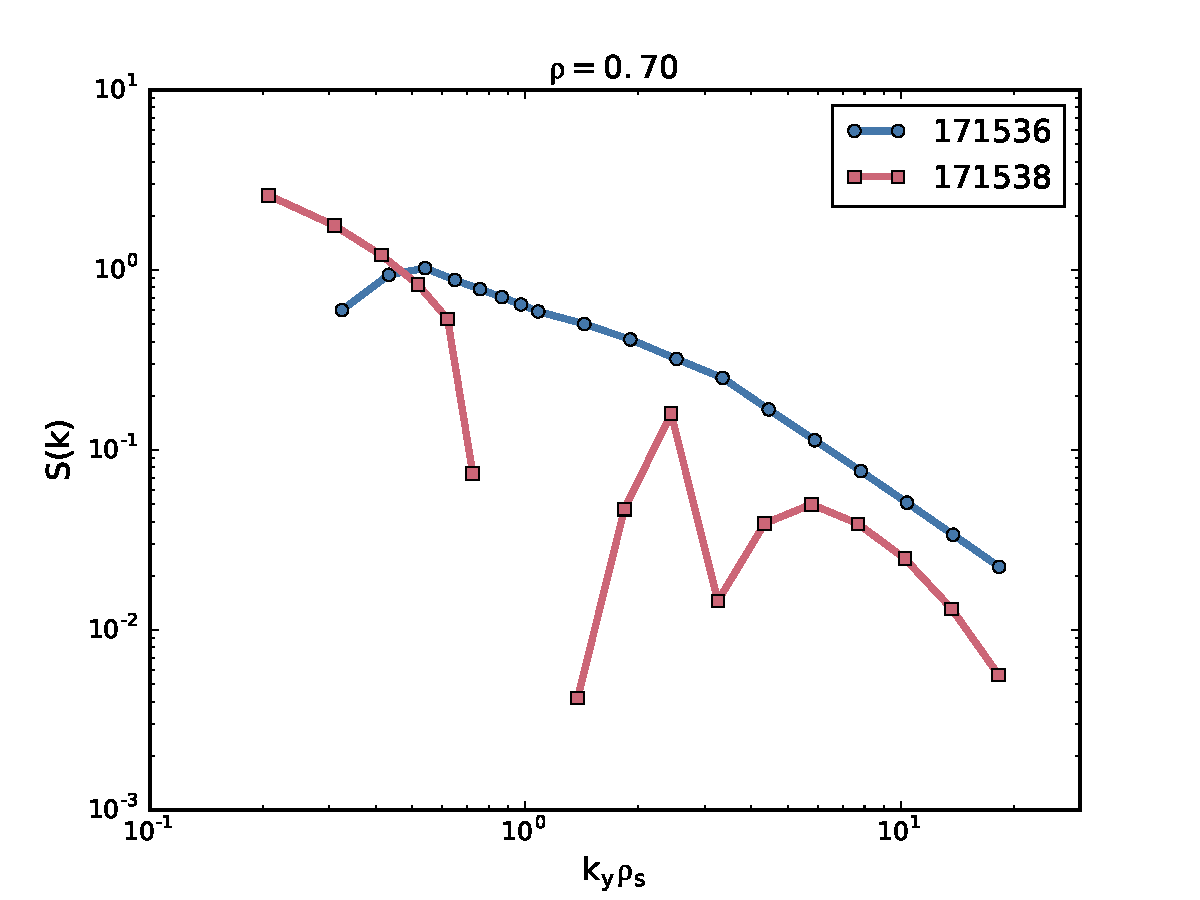
\includegraphics[width = \textwidth]{%
    Chapters/TurbulenceMeasurements/figs/density_spectra.pdf}
  \caption[TGLF-predicted density-fluctuation spectra at $\rho=0.7$]{%
    TGLF-predicted density-fluctuation spectra at $\rho=0.7$.
    Note that only $171536$ uses SAT\_RULE $= 1$,
    which is calibrated against multiscale GYRO results;
    $171538$ uses SAT\_RULE $= 0$.
    Thus, it is difficult to draw conclusions\ldots
  }
\label{fig:TurbulenceMeasurements:density_spectra}
\end{figure}


\bibliographystyle{plainurl}
\bibliography{references}
